\section*{Описание экспериментальной установки}

\begin{figure}[H]
	\centering
	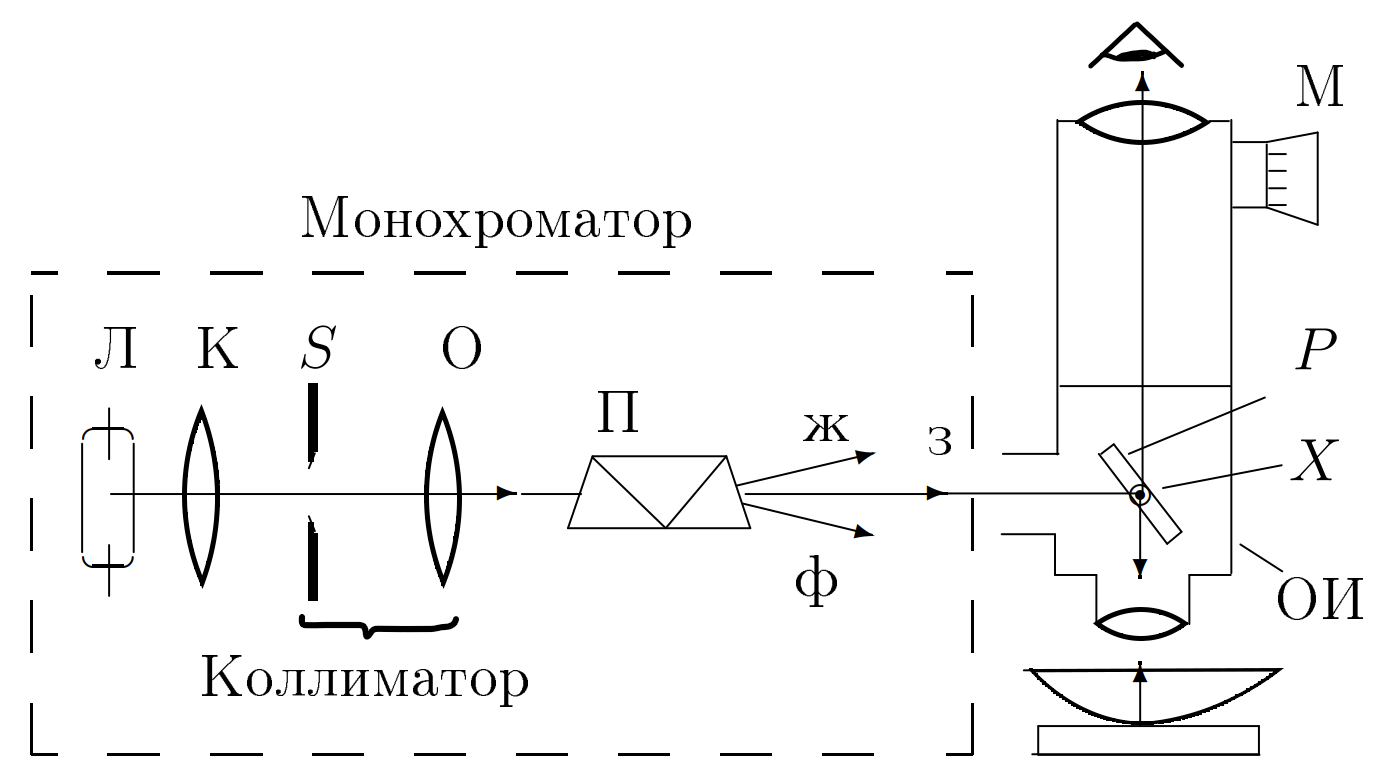
\includegraphics[width=0.45\textwidth]{../Изображения/Установка.png}
	\caption{Схема экспериментальной установки}
\end{figure}

Белый свет от ртутной лампы попадает на призменный монохроматор, состоящий из конденсора(К), коллиматора(щели S и объектива O), и призмы прямого зрения(П). После монохроматора свет попадает на расположенный между объективом и окуляром микроскопа опак-иллюминатор(ОИ), внутри которого находится полупрозрачная стеклянная пластинка(P), наклоненная под углом 45° к оптической оси микроскопа. Свет частично отражается от пластинки и попадает на исследуемую линзу. 